Una barra metálica de \qty{100}{\centi\metre} de longitud tiene sus
extremos $x=0$, $x=100$ mantenidos a \qty{0}{\degreeCelsius}.
Inicialmente, la mitad de la barra está a \qty{60}{\degreeCelsius};
mientras que la otra mitad a \qty{40}{\degreeCelsius}.
Asumiendo un coeficiente de difusividad de \num{0.16} unidades c.g.s
y un entorno aislado.

\begin{parts}
	\part\label{1a}

	Describa la ecuación diferencial correspondiente, así como las
	condiciones iniciales y de frontera.

	\part

	No resuelva, solo comente los pasos a tener en cuenta para resolver
	el problema en el ítem~(\ref{1a}).
\end{parts}

\begin{figure}[ht!]
	\centering
	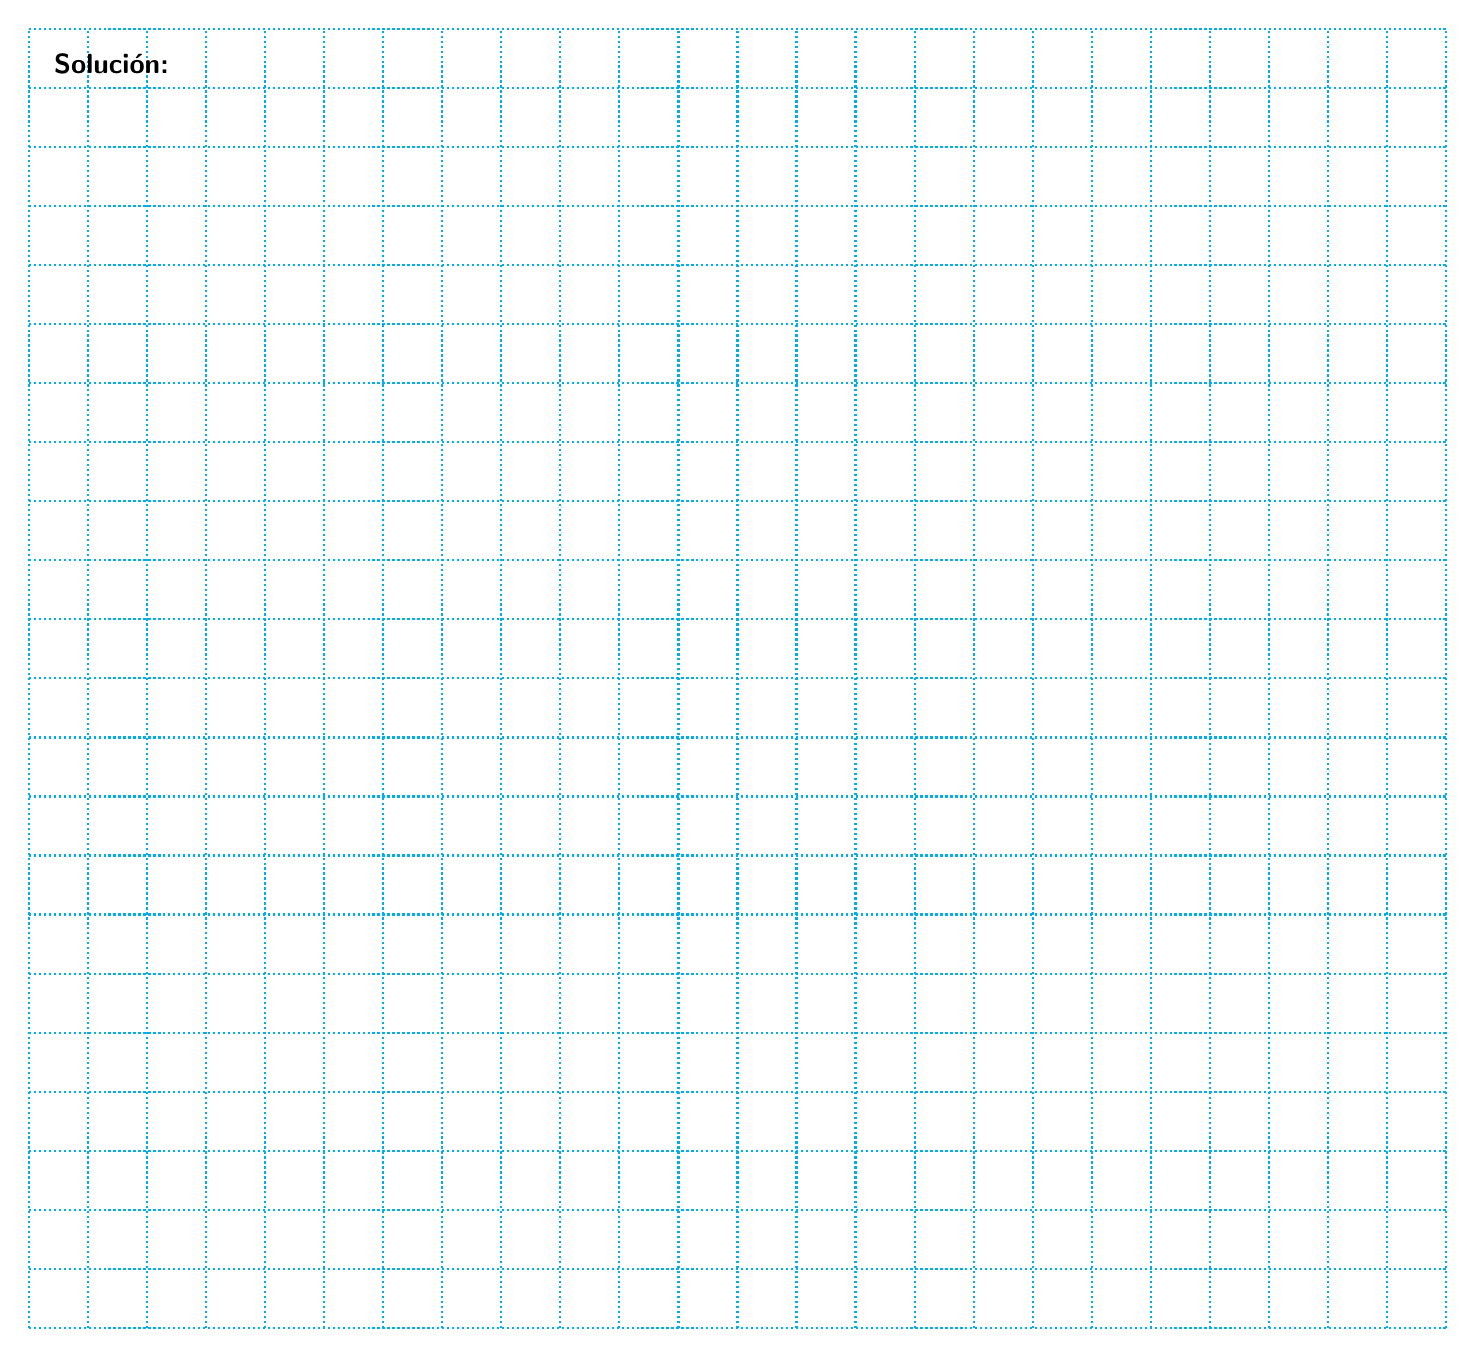
\begin{tikzpicture}[xscale=0.75,yscale=0.75]
		\draw[help lines,color=cyan,thick,densely dotted] (0,0) grid (24,22);
		\draw (1.4,21.4) node {\textsf{\bfseries Solución:}};
	\end{tikzpicture}
\end{figure}
